%%%%%%%%%%%%%%%%%%%%%%%%%%%%%%%%%%%%%%%%%%%%%%%%%%%%%%%%%%%%%%%%%%%%%%%
%%%%%%%%%%%%%%%%%%%%%%%%%%%%%%%%%%%%%%%%%%%%%%%%%%%%%%%%%%%%%%%%%%%%%%%
%%%%%                                                                 %
%%%%%     07_results.tex                                              %
%%%%%                                                                 %
%%%%% Author:      <Renzo Andri>                                      %
%%%%% Created:     <Dec 14, 2013>                                     %
%%%%% Description: ...                                                %
%%%%%                                                                 %
%%%%%%%%%%%%%%%%%%%%%%%%%%%%%%%%%%%%%%%%%%%%%%%%%%%%%%%%%%%%%%%%%%%%%%%
%%%%%%%%%%%%%%%%%%%%%%%%%%%%%%%%%%%%%%%%%%%%%%%%%%%%%%%%%%%%%%%%%%%%%%%

\chapter{Results}
The goal of this thesis was a redesign of the already existing OpenRISC implementation\cite{website:OpenCores}. This implementation will be called \textit{"original"} in the following chapter. The original implementation has already been optimized and will be refered as the \textit{"optimized"} implementation. Both of these implementations were synthesized with the same setup as our implementation to guarantee for comparable data.
\section{Throughput Comparison}
To compare different processor architectures different performance measures can be used. When comparing different processors the frequency can be compared. This criteria is highly dependent on the number of pipeline stages and does not consider how many and which instruction was executed in each cycle.
Therefore, the first performance measure we used is \gls{ipc} which ratioes the number of effective executed instructions to the number of cycles needed to execute them. An optimal \gls{ipc} in a single-cycle RISC architecture would be 1, but this value cannot be reached by a pipelined architecture because at the end all final instructions have to pass all pipeline stages: With four stages as we used, there are always three additional cycles to finish execution. "No operation" (l.nop) which are usually injected by compiler\footnote{An example why the OpenRISC compiler reasonably adds a l.nop is the delay slot after a jump instruction. The instruction which follows a jump instruction is executed in the so-called delay slot, usually the compiler tries to reorder the operations such that an expendient instruction is put into the delay slot. If this was not possible due to some dependency, the compiler adds a l.nop instead.} are not counted as effective executed instructions and decrease IPC. The main source of a decreased IPC are stalls. Equations \ref{equ:ipc}\footnote{$\mathbbm{1}$ stands for the indicator function: $\mathbbm{1}_{condition}=\begin{cases}
								1 & \text{condition fullfilled},\\
								0 & \text{else}.
							    \end{cases}$} and \ref{equ:ipc2} show a formal description of the used IPC calculation.
\begin{equation}
\label{equ:ipc} 
IPC=\frac{\#instructions}{\#cycles}=\frac{\sum_{k=k_{start}}^{k_{end}} \mathbbm{1}_{(Instr[k]\ne'nop' \wedge PC[k]\ne PC[k-1])}}{3+(k_{end}-k_{start}+1)}
\end{equation}
\begin{equation}
\label{equ:ipc2} 
IPC=\frac{\#instructions}{\#cycles}=\frac{(k_{end}-k_{start}+1)-\#nop-\#stalls}{3+(k_{end}-k_{start}+1)} 
\end{equation}

Table \ref{tab:ipc} shows \gls{ipc} values of OR10N for seven sample programs and Table \ref{tab:ipc_comp} compares the resulting \gls{ipc} with them from the original and optimized implementation. The sample programs were chosen such that all kinds of operations are covered: These are branch, computation and storage intensive functions.
\begin{table}[htbp]
 \caption{IPC for sample programs on OR10N}
 \label{tab:ipc}
\centering\begin{tabular}{|l|r|r|r|r|r|} \hline
program name & \#instr. & \#nop & \#stalls & \#cycles & \gls{ipc} \\ \hline
fullCoverage.S   & 336  & 31 &    20 &    390 & 0.8615 \\ \hline
matrixMul.c    & 5'537  & 10 &   512 &  6'062 & 0.9134 \\ \hline
matrixAdd.c    & 5'341  & 15 &     0 &  5'359 & 0.9966 \\ \hline
stencil.c      & 1'656  & 44 &   111 &  1'814 & 0.9129 \\ \hline
towerofHanoi.c& 88'209  & 56 & 2'048 & 90'316 & 0.9767 \\ \hline
fibonacci.c    & 3'536 & 223 &    10 &  3'772 & 0.9374 \\ \hline
bubblesort.c &  70'704 & 101 & 4'950 & 75'758 & 0.9333 \\ \hline
\end{tabular}
\end{table}


\begin{table}[htbp]
 \caption{Comparison of IPC}
 \label{tab:ipc_comp}
\centering\begin{tabular}{|l|r|r|r||r|r|} \hline
program & original & optimized & OR10N & \multicolumn{2}{c|}{Improvement} \\ \cline{1-4} \cline{5-6}
matrixMul.c & 0.5458 & 0.9996 & 0.9134 & +83.14\% & +67.35\% \\ \hline
matrixAdd.c & 0.6697 & 0.9960 & 0.9966 & +48.72\% & +48.81\% \\ \hline
stencil.c & 0.6095 & 0.9572 & 0.9129 & +57.05\% & +49.78\% \\ \hline
towerofHanoi.c & 0.6143 & 0.9773 & 0.9767 & +59.09\% & +58.99\% \\ \hline
fibonacci.c & 0.5695 & 0.9101 & 0.9374 & +59.81\% & +64.60\% \\ \hline
bubblesort.c & 0.6484 & 0.9329 & 0.9333 & +43.88\% & +43.94\% \\ \hline\hline
Mean \o & 0.6095 & 0.9622 & 0.9451 & +57.86\% & +55.04\% \\ \hline
\end{tabular}
\end{table}

As expected the optimized and our implementation are 57 \% and 55 \% better than the original one. The main reasons are the longer latency of the multiplication, which lasts four cycles in the original implementation instead of two, which results in more stalls than in the optimized and in our implementation. The comparison between our implementation and the optimized shows some benefit for the optimized implementation. Mainly because multiplications can be more efficiently executed due to aditional write ports at the \gls{gpr}. This increases the area and setup delay of the \gls{gpr}.  \\ \\

An even better performance measure is \gls{ops}, or \gls{mops} which indicates how many effective executed instructions are executed in one second. This measure can easily be determined with \gls{ipc} and the maximal clock frequency. Equation \ref{equ:ops} and \ref{equ:mops} shows this relation. 

\begin{equation}
\label{equ:ops}
\Theta_{OPS} = IPC \cdot f_{clk}= \frac{IPC}{T_{clk}}
\end{equation}
\begin{equation}
\label{equ:mops}
\Theta_{MOPS} = \Theta_{OPS} \cdot \left( \frac{10^{-6}\ MOPS}{1\ OPS}\right)
\end{equation}

Table \ref{tab:ops_cmp} and diagram \ref{fig:results} compare the throughput in \gls{mops} of the three implementations of the sample programs. The white part of the bars indicates the difference of the actual \gls{ipc} to an optimal IPC of 1. The original architecture is shown in red, the optimized one in blue and the OR10N architecture in green.

\begin{table}[htbp]
 \caption{Throughput comparison in MOPS}
 \label{tab:ops_cmp}
\centering\begin{tabular}{|l|r|r|r||r|r|} \hline
program & original & optimized & OR10N & \multicolumn{2}{c|}{Improvement} \\ \hline
matrixMul.c & 184.39 & 305.69 & 333.36 & +65.78\% & +80.79\% \\ \hline
matrixAdd.c & 226.25 & 304.59 & 363.72 & +34.62\% & +60.76\% \\ \hline
stencil.c & 205.91 & 292.72 & 333.18 & +42.16\% & +61.80\% \\ \hline
towerofHanoi.c & 207.53 & 298.87 & 356.46 & +44.01\% & +71.76\% \\ \hline
fibonacci.c & 192.40 & 278.32 & 342.12 & +44.66\% & +77.82\% \\ \hline
bubblesort.c & 219.05 & 285.29 & 340.62 & +30.24\% & +55.50\% \\ \hline\hline
Mean \o & 205.92 & 294.25 & 344.91 & +42.89\% & +67.49\% \\ \hline
\end{tabular}
\end{table}

Due to the higher maximal frequency of the proposed implementation, an even higher throughput is achieved compared to the original implementation. OR10N achieves 17 \% higher throughput than the optimized implemenation because of the shorter longest path, a comparison of the maximal frequencies and areas are showed in Table \ref{tab:area_cmp}. Section \ref{sec:area} shows detailed information about the area distribution of OR10N.

\begin{figure}[t!]
\centering
%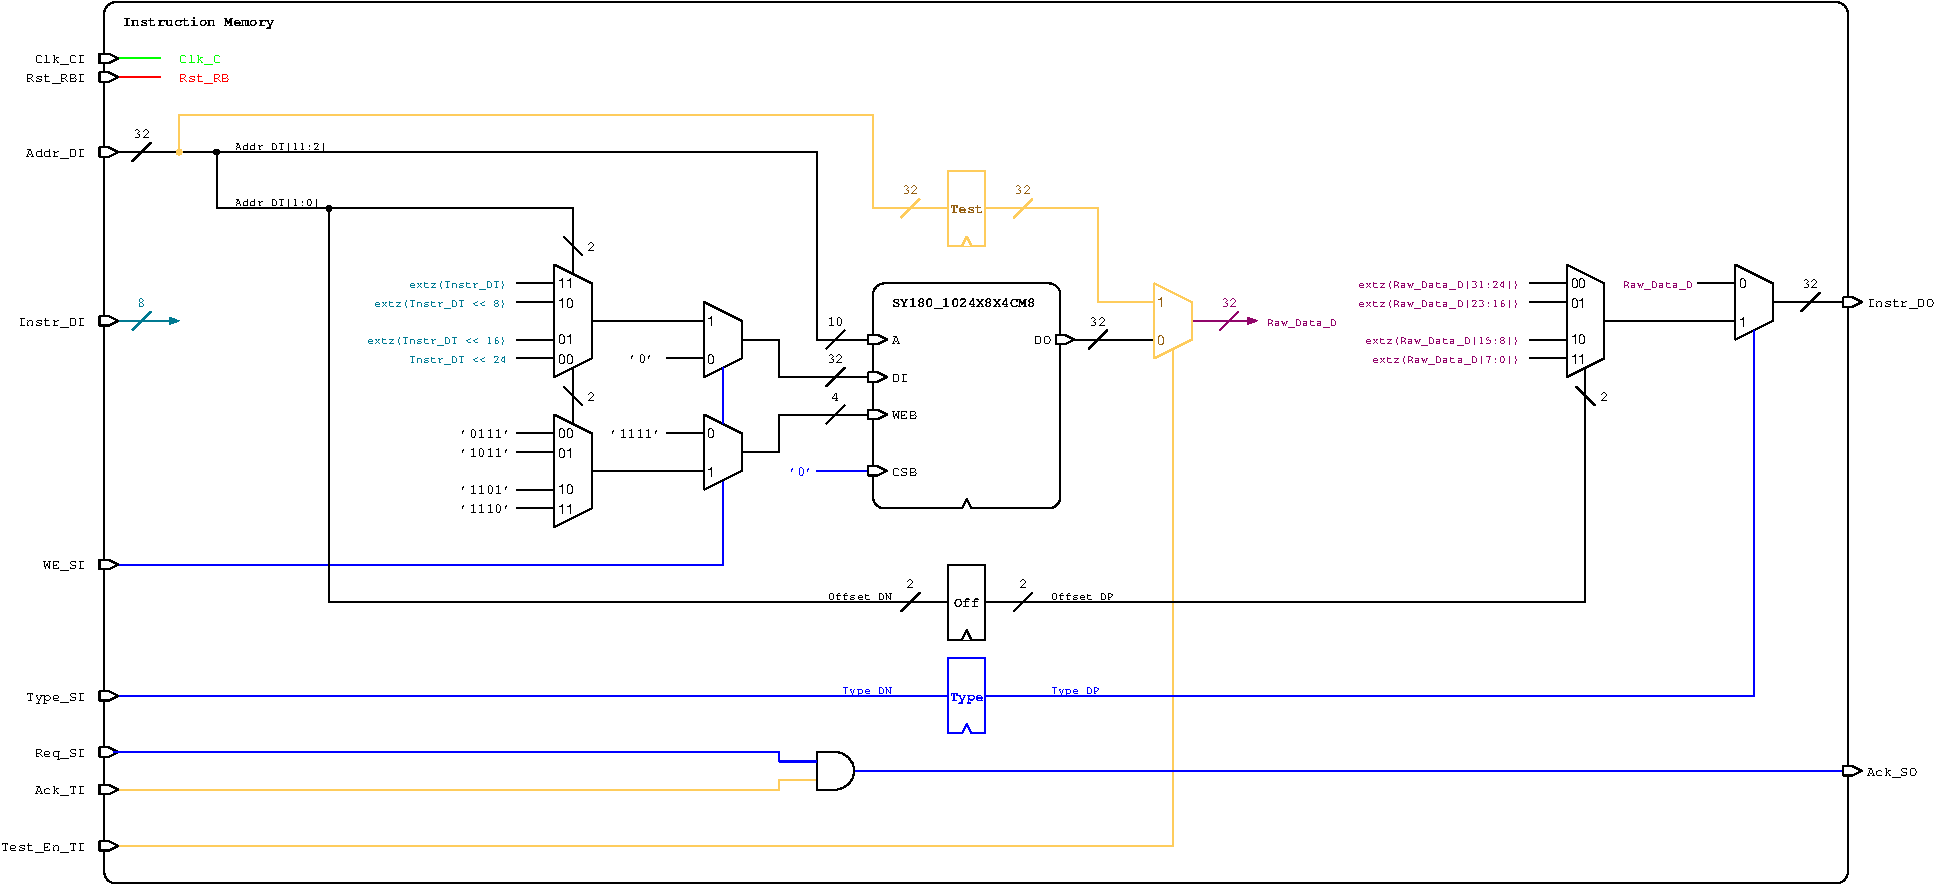
\includepdf{figures/instr_mem.pdf}
\includegraphics[scale=0.6]{figures/results.png}
\caption{Comparison between OR10N, original and optimized architecture. TODO: replace!!}
\label{fig:results}

\end{figure}

\begin{table}[htbp]
 \caption{Area and frequency comparison}
 \label{tab:area_cmp}
\centering\begin{tabular}{|r|r|r||r|r|} \hline
implementation & \multicolumn{2}{c||}{area} & \multicolumn{2}{c|}{$f_{max}$} \\ \hline
original & 755'608 $\mu m^2$ & $-$ & 337.84 MHz & $-$ \\ \hline
optimized & 789'090 $\mu m^2$ & $+$4.43 \% & 305.81 MHz & $-$9.48 \% \\ \hline
OR10N & 779'200 $\mu m^2$ & $+$3.12 \% & 364.96 MHz & $+$8.03 \% \\ \hline
\end{tabular}
\end{table}




